\documentclass[tikz,border=10pt]{standalone}
\usepackage{circuitikz}
\usepackage{xcolor}
\usepackage{amsmath}
\usetikzlibrary{arrows}

\begin{document}
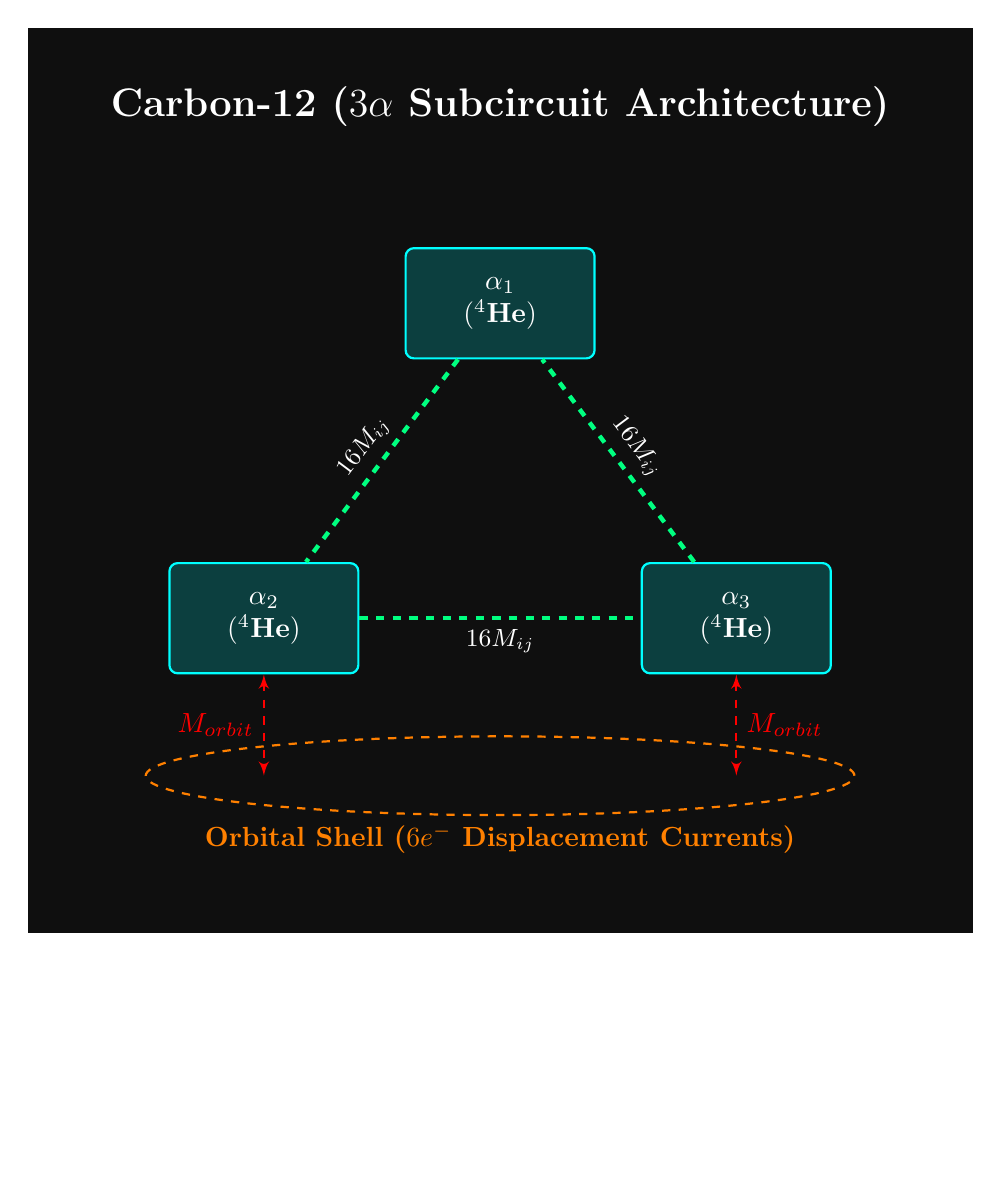
\begin{tikzpicture}[>=latex']

\definecolor{neonblue}{RGB}{0, 255, 255}
\definecolor{neongreen}{RGB}{0, 255, 128}
\definecolor{darkbg}{RGB}{15, 15, 15}
\definecolor{neonpurple}{RGB}{200, 0, 255}

% Fill background
\fill[darkbg] (-6,-6) rectangle (6,5.5);

% Title
\node[text=white, font=\bfseries\Large] at (0, 4.5) {Carbon-12 ($3\alpha$ Subcircuit Architecture)};

\tikzset{
    alpha block/.style={
        draw=#1, thick, fill=darkbg!80!#1,
        rectangle, rounded corners=3pt,
        minimum width=2.4cm, minimum height=1.4cm,
        text=white, font=\bfseries, align=center
    },
    bus/.style={
        draw=neongreen, ultra thick, dashed
    }
}

% 3 ALPHAS (Equilateral Triangle planar projection)
\node[alpha block=neonblue] (Top) at (0, 2) {$\alpha_{1}$\\$(^4\text{He})$};
\node[alpha block=neonblue] (BL) at (-3, -2) {$\alpha_{2}$\\$(^4\text{He})$};
\node[alpha block=neonblue] (BR) at (3, -2) {$\alpha_{3}$\\$(^4\text{He})$};

% --- MACRO-COUPLINGS (BUS LINES) ---
\draw[bus] (Top) -- (BL) node[midway, sloped, above, text=white, font=\small] {$16 M_{ij}$};
\draw[bus] (BL) -- (BR) node[midway, sloped, below, text=white, font=\small] {$16 M_{ij}$};
\draw[bus] (BR) -- (Top) node[midway, sloped, above, text=white, font=\small] {$16 M_{ij}$};

% Orbital Displacement current representation
\draw[color=orange, dashed, thick] (0,-4) ellipse (4.5cm and 0.5cm);
\node[color=orange, align=center, font=\bfseries] at (0, -4.8) {Orbital Shell ($6e^-$ Displacement Currents)};

\draw[<->, dashed, red, thick] (BL) -- (-3, -4) node[midway, left] {$M_{orbit}$};
\draw[<->, dashed, red, thick] (BR) -- (3, -4) node[midway, right] {$M_{orbit}$};

% Legend
\node[text=white, text width=9cm, align=center, draw=white, dashed, inner sep=8pt] at (0, -7.5) {
    \textbf{IC-Equivalent Topology Level}\\
    Each $\alpha$ macro-block encapsulates a synchronized 4-nucleon LC mesh.\\
    Bus lines represent 16 cross-coupled inductive pairs between blocks.\\
    \textit{Total Carbon-12 Network: 66 discrete connections.}
};

\end{tikzpicture}
\end{document}
